	\documentclass[french, 12pt]{report}
\usepackage[latin1, utf8]{inputenc}
\usepackage{color}
\usepackage{graphicx}
\usepackage{listings}
\usepackage{amssymb}
\usepackage{amsmath}
\usepackage{pstricks}
\usepackage{enumitem}
\usepackage{multicol}
\usepackage{verbatim}
\usepackage{listings}
\usepackage{tikz}
\usetikzlibrary{arrows,automata}
\usetikzlibrary{shapes,snakes}
\usepackage{pgfplots}
\usepackage{pgfplotstable}
\usepackage{xifthen}
\usepackage{fancyhdr}
\usepackage{caption}
 
%%\pgfplotsset{compat=1.16}
\setlist[description]{leftmargin=\parindent,labelindent=\parindent}

\definecolor{gray}{rgb}{0.4,0.4,0.4}
\definecolor{darkblue}{rgb}{0.0,0.0,0.6}
\definecolor{cyan}{rgb}{0.0,0.6,0.6}
\definecolor{darkgreen}{RGB}{0,150,0}
 	
\newcommand{\cblue}[1]{ \textcolor{blue}{#1}}
\newcommand{\corange}[1]{ \textcolor{orange}{#1}}
\newcommand{\cviolet}[1]{ \textcolor{violet}{#1}}
\newcommand{\crouge}[1]{ \textcolor{red}{#1}}
\newcommand{\cvert}[1]{ \textcolor{darkgreen}{#1}}
\newcommand{\cgris}[1]{ \textcolor{gray}{#1}}

%% ------------------------- Header Footer
\pagestyle{fancy}
\fancyhf{}
\fancyhead[LE,RO]{OCR}
\fancyhead[RE,LO]{ }
\fancyfoot[CE,CO]{\leftmark}
\fancyfoot[LE,RO]{\thepage}
% -------------------------- END Header Footer

%% ------------------------- Formular
\newcommand{\cformular}[2]{
\begin{center} 
\begin{description} 
\item[#1] #2 
\end{description} 
\end{center}
}
%% ------------------------- END Formular

%% ------------------------- RO Model
\newcommand{\rovarinout}[5]{
\begin{description}
\item[La variable entrante sera] #1
\item[La variable sortante sera] #2 car:
\end{description}
\begin{multicols}{3}
#3, #4, #5
\end{multicols}
}

\newcommand{\romodel}[8]{
\begin{multicols}{2}
[Voici le nouveau modèle:]
\begin{description}
\item[Déterminer] #1
\item[#2] #3 % ((2) maximisant | minimisant )
\item[Variables hors base] #4
\item[Variables de Base] #5
\item[Solution admissible] #6 et Z = #7
\end{description}
#8 % contraintes
\end{multicols}
}
%% ------------------------- END RO Model

%% ------------------------- XML

\lstset{
  basicstyle=\ttfamily,
  columns=fullflexible,
  showstringspaces=false,
  commentstyle=\color{gray}\upshape
}

\lstdefinelanguage{XML}
{
  morestring=[b]",
  morestring=[s]{>}{<},
  morecomment=[s]{<?}{?>},
  stringstyle=\color{black},
  identifierstyle=\color{darkblue},
  keywordstyle=\color{cyan},
  morekeywords={xmlns,version,type}% list your attributes here
}
%% ------------------------ END XML

%% ------------------------ Almost all
\newcommand{\almost}{\mid\kern-0.40em{\backsim}\ }
%% ------------------------ END Almost all

%% ------------------------ Inverse DL lite
\newcommand{\inverse}{\urcorner\ }
%% ------------------------ End Inverse DL lite

%% ------------------------ Python code for Machine leaning
\definecolor{codegreen}{rgb}{0,0.6,0}
\definecolor{codegray}{rgb}{0.5,0.5,0.5}
\definecolor{codepurple}{rgb}{0.58,0,0.82}
\definecolor{backcolor}{rgb}{0.97,0.97,0.95}

\lstdefinestyle{mlpythoncode}{
    backgroundcolor=\color{backcolor},   
    commentstyle=\color{codepurple},
    keywordstyle=\color{codegreen},
    numberstyle=\tiny\color{codegray},
    stringstyle=\color{magenta},
    basicstyle=\footnotesize,
    breakatwhitespace=false,         
    breaklines=true,                 
    captionpos=b,                    
    keepspaces=true,                 
    numbers=left,                    
    numbersep=5pt,                  
    showspaces=false,                
    showstringspaces=false,
    showtabs=false,                  
    tabsize=2,   
    emph={[2]sklearn, model_selection, train_test_split,KFold, linear_model, LinearRegression, LogisticRegression,
    DecisionTreeRegressor, tree, neighbors, KNeighborsClassifier, svm, SVC, metrics, confusion_matrix,precision_recall_fscore_support,
    LeaveOneOut},
	emphstyle=[2]\color{blue}
}

\newcommand{\sepline}{\textcolor{gray}{\noindent\rule{14cm}{0.1pt}}}
\newcommand{\paramtype}[1]{\textcolor{gray}{\textsf{\textit{#1}}}}

\newcommand{\funcdoc}[4]{
	\ \\
	\textit{\textsf{\cblue{#1}}}
    \ifthenelse{\isempty{#2}}%
    {}%
	{    \ \\\sepline\ \\
	\textbf{Paramètres}
	{#2}}
    \ifthenelse{\isempty{#3}}%
    {}%
	{    \ \\\sepline\ \\
	\textbf{Retourné}
	{#3}}
    \ifthenelse{\isempty{#4}}%
    {}%
	{    \ \\\sepline\ \\
	\textbf{Méthodes}
	{#4}}
}

%% ------------------------ END Python code

%% ------------------------ FORMULA
\newcommand{\formula}[1]{
\begin{center}
{#1}
\end{center}
}
%% ------------------------ END FORMULA


%% ------------------------ FORME SHAPE
\newcommand{\cshape}[2]{
\begin{center}
\scalebox{#1}{#2}
\end{center}
}
%% ----------------------- END FORME SHAPE

%% ------------------------- AUTHORS
\newcommand{\cauthors}[1]{\textit{#1}}
%% -------------------------

\begin{document}

\begin{titlepage}
\begin{center}
       \vspace*{1cm}
 
       \scalebox{2.5}{\textbf{Reconnaissance Optique}}
       \scalebox{2.5}{\textbf{des Caractères}}
 
       \vspace{0.5cm}
       \scalebox{2}{Master 2 IA}
 
       \vspace{1.5cm}
 
       \textbf{LAURENT Thomas}
 
       \vfill
 
       \vspace{0.8cm}
 
       Années: 2018 - 2019
 
   \end{center}
\end{titlepage}
\pagebreak
\pagebreak
\pagebreak
\tableofcontents
\pagebreak

\part{Introduction}
\chapter{Introduction Générale}
\pagebreak

Depuis les années 1950, on parle d'intelligence artificielle (IA, ou AI en anglais) un programme ayant les capacités de penser ou de raisonner comme un processus qui serait humainement exécuté à l'aide d'une conscience ou un réseau neuronal. Un mécanisme pensant pouvant prédire une action, un état ou un résultat. Mais l'intelligence artificielle est en réalité plus complexe, un processus pouvant donner des résultats sur des données qu'elle connait, donc que l'algorithme connait à l'avance le résultat, ce n'est pas un processus d'intelligence artificielle car elle ne fait que pour un dictionnaire de données retourner la valeur associée aux datas donnés. \\
Pour qu'un processus soit dit, doté d'une intelligence, il faut qu'il soit équipé d'une capacité de raisonnement voir d'apprentissage pour les cas où les données en entrée lui soit totalement inconnue, dans ce cas là, il doit savoir prédire une réponse fiable et ayant du sens en utilisant les données qu'il connait déjà.\\
\linebreak
Le domaine de l'intelligence artificielle est bien plus vaste que la description donnée ci dessus, selon le \textit{Texte de la 236e conférence de l'université de tous les savoirs donné par Jean-paul HALTON} il existerait trois grandes approches de celui-ci, l'approche \emph{Symbolique}, l'approche \emph{Connexioniste} puis l'approche \emph{Statistique}, je vais les décrire ci-dessous.

\pagebreak
\section{L'approche symbolique}

Un exemple réel d'approche symbolique, le code de la route, chaque panneau (ou inscription qu'elle soit au sol ou en hauteur) ont une signification spécifique sur l'état que l'automobiliste doit adopter sur sa façon de conduire ou dans un état future. Si un automobiliste voit un panneau <sens interdit> sur un tronçon juste devant lui, une information est envoyé au cerveau (où plutôt dans la base de connaissance) et une réponse direct (sans aucun apprentissage) est retournée par le réseau de connaissance indiquant qu'il lui ai interdit de continuer sa route sous resserve d'accidents par exemple.\\
Cette approche est dite \textit{offline}  car avant d'effectuer des requêtes à la base de connaissance celle-ci a besoin d'être au préalable remplit d'informations vrais et dans touts les cas possible. Admettons qu'un conducteur n'ai pas apprit la signification d'un panneau <sens interdit> voyer vous le problème que cet individu peut causer.\ L'hypothèse du monde clos est appliqué par cette approche, pour une donnée que le réseau de connaissance ne connais pas, la réponse retournée sera une réponse négative, prenons encore notre conducteur ci dessus, si celui ci voit un nouveau tronçon devant lui (un tronçon qu'il n'a jamais vue), il n'a aucune données dans sa base de connaissance qui décrit ce nouveau tronçon (bien-sur nous allons admettre que le conducteur n'a pas la possibilité d'ajouter de nouvelles informations dans sa base de connaissance ni d'apprendre sur ce nouveau tronçon), le conducteur va trivialement dire qu'il ne va pas s'aventurer sur ce nouveau tronçon car, sa base de connaissance ne lui a fournit aucune information. \\
\linebreak
Dans l'informatique, nous le savons, les ordinateurs ne savent que faire des opérations logiques simple comme le ET, le OU, et le NOT, ces opérations sont accompagnés de registres (mémoire vive, disque dur, ...) pouvant pour la durée de la vie d'un processus stocker les données et faire des opérations dessus avec d'autres données stocké dans la machine, c'est à partir de là que quelques registres et une succession d'opérations logiques simple que l'on peut former des circuits pouvant traiter les opérations mathématiques comme l'addition, la soustraction, la multiplication et la division. Ses informations sont possibles car, elles sont ancré dans la base de connaissance de la machine qui lance les processus, par héritage les processus sont capables d'appeler les circuits pouvant faire les opérations cité ci dessus. \\ Un exemple logiciel d'approche symbolique serait le langage \textit{Prolog} qui pour une base de connaissance donné en début de fichier, infère les différentes questions posées dans la suite du programme.\\ Prenons un exemple simple, pour une base de connaissance donné ci dessous:
\linebreak
\lstset{style=mlpythoncode}
\begin{lstlisting}[language=Prolog]
- Homme(Jean)
- Homme(Pierre)
- Femme(Marie)
- En_couple(Jean,Marie)
\end{lstlisting}
\ \\
Effectuons des requêtes à la base de donnée ci dessus, demandons:
\begin{description}
\item[] Est ce que Jean, est un homme? la base de connaissance va répondre oui.
\item[] Est ce que Marie, est un homme? non.
\item[] Est ce que Marie et Pierre, sont en couple? non.
\item[] Est ce que Jean et Marie sont en couple? oui.
\end{description}

Pour confirmer la théorie du monde clos, nous pouvons demander si Philippe est un homme, n'ayant aucune information sur ce dénommé Philippe, la base de connaissance va déclencher une exception disant qu'il n'a pas trouvé un tel Philippe, car il ne connait pas ce Philippe, la base de connaissance va répondre NON.\\ 
\linebreak L'hypothèse du monde clos est une échappatoire fréquemment utilisé dans les bases de connaissances, mais le non envoyé à cause de cette hypothèse n'a pas la même signification que le non Philippe n'est pas un homme. Pour y remédier certains logiciels ont ajouté une valeur à "oui" et "non", nous appelons ceci le \textit{Three valued logic} et ce mode est implémenté dans certaines bases SQL, la troisième valeur est nommé "unknow" ayant la bonne signification demandé par l'hypothèse du monde close.

\pagebreak
\section{L'approche connexionniste}
L'approche connexionniste est l'approche la plus proche du schéma du cerveau au vue des requêtes. Le processus de réflexion du cerveau est représenté par une série de mini processus ne pouvant répondre qu'a un type de problème qui est définit lors de la création de ce mini processus, un mini processus est nommé neurone dans le cerveau, et nous allons préférer l'utilisation du terme neurone pour la suite. \\
Chaque neurone est définit par plusieurs entrées, et une seule sortie et peu être semblable à un \textit{Perceptron} en machine learning:

\begin{center}
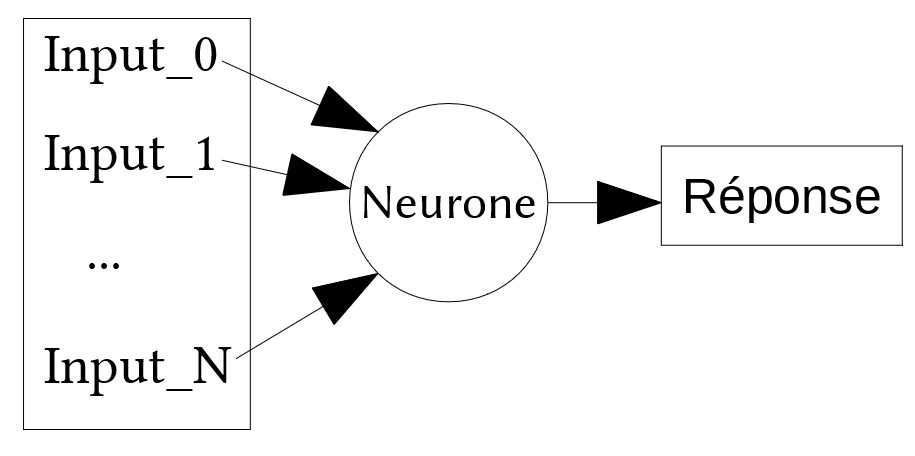
\includegraphics[scale=0.3]{img/neurone.jpg} 
\end{center}

En informatique, chacun de ses neurones sont équipé d'une capacité d'apprentissage qui va influer sur les futures résultats, via un vecteur de variables (dites Poids ou weight en anglais) ce sont ses variables couplé aux données d'entré (via un dot) qui va donner le résultat de l'opération, lors de la période de création du neurone, il se voit attribuer son vecteur de poids à des valeurs aléatoire (plus généralement que des zero), une base de connaissance de référence,  une fonction de résultat, et d'une fonction d'erreur pour donner une signification future au vecteur de poids.\\
\linebreak
Chaque sample (ou ligne) de la base de connaissance de référence est doté d'une variable réponse (noté étiquette) indiquant la réponse que le neurone devrait donner si dans le future on lui demande le résultat de ce sample. Avant de rendre le neurone fonctionnel, il se doit de passer les tests d'apprentissages, pour chaque sample dans la base de connaissance de référence, il va le multiplier avec le vecteur de poids et en tirer le résultat via une fonction de résultat et calculer l'indice d'erreur avec le résultat donné et la variable étiquette du sample, via l'indice d'erreur les poids du neurone vont s'équilibrer jusqu'à converger vers un vecteur dit optimal. Une fois optimal ce neurone donnera les meilleurs résultats qu'il pourra donner.\\
\linebreak
Les résultats données par le neurone ne sont pas fiable à 100\%, il se peut, qu'il y ai des faux positif qui passent pour de vrai négatif, mais nous en discuterons plus bas dans ce rapport.

\pagebreak
\section{L'approche statistique}

L'approche statistique se base sur les statistiques, prenons un exemple d'une grande chaine de distribution, celle ci a des besoins plus ou moins conséquent d'innover pour continuer à avoir une trace dans les têtes des consommateurs, pour s'y faire le staff organise des études sur leur site internet, ses études sont à compléter de chiffres et de choix prédéfinit. Une fois équipé de beaucoup de résultats, il s'en vient de la prise de décision sur les futures changements, l'entreprise munit d'un arbre de décision le remplit selon les valeurs généré par l'étude. pour chaque nœud de l'arbre, l'entreprise va devoir entreprendre une action (peindre, commander, offrir ....), sur les feuilles de l'arbre le gain (ou la perte) prévue en hypothèse, et entre deux nœuds la probabilité calculer avec l'étude.\\
\linebreak
Une autre approche statistique largement utilisé est via les réseau bayésien. Les enfants qui trient leurs bonbons en faisant une pile de bonbon qu'ils aiment, une pile de bonbon qu'ils n'aiment pas puis une pile de bonbon qu'ils se savent pas quoi en penser. Sur l'arrière du paquet il est indiqué le gout du bonbon par rapport à la forme, la couleur et la taille (l'axiome de bijection n'est pas satisfait). Dans un premier temps l'enfant va pour chaque bonbon qu'il prend lire l'arrière du paquet puis classe le bonbon dans une pile, à force de voir les piles de bonbon grossir, il décide de laisser tomber le paquet de bonbon pour classer la suite de lui même, ainsi pour chaque bonbon prit, il calculera une sorte de probabilité avec ses croyances et l'état actuel des piles. Le cerveau est très complexe pour pouvoir introduire ce raisonnement dans un processus, il existe donc des versions mathématiques du calcule de l'appartenance d'un bonbon à une pile, par exemple \textit{l'entropie} ou le \textit{le gain d'information}.\\

\pagebreak

Selon moi, ses trois approches forme une définition simple de l'intelligence artificiel, mais plusieurs approches qui ne sont pas cité ci dessus ont leur place dans la définition, car rien qu'avec les trois approches ci dessus nous pouvons inférer sur une base de donné en posant des questions simple, généraliser un concept en une série de matrice et prédire des événements selon une base de croyance. Enfin, l'une des approches que je voudrais ajouter est cité un peu plus haut dans l'approche statistique, l'autre approche est aussi basé sur des inférences sur une base de donné, non pour donner une réponse seulement boolean, mais pour fournir tout un modèle en guise de réponse.

\section{L'approche décisionnel}

La prise de décision, une brique très utilisé dans beaucoup de processus se disant intelligent, là où un système de recommandation trie les films selon des probabilités allié à un algorithme de \textit{ranking}, il n'y a rien de vraiment décisionnel. Un processus devant prendre des décisions est un processus qui veut maximiser son gain ou minimiser sa perte. Un joueur d'échec cherche à maximiser son gain pour faire perdre son adversaire, c'est un jeu à somme nul, la somme des gains du gagnant et du perdant donne zero. Pour cela, il nous faut une décomposition des possibilités que les deux joueurs peuvent faire puis construire une matrice qui pour chaque lignes numéroté par un choix que le joueur 1 peut faire, pour chaque colonnes par un choix que le joueur 2 peut faire et pour chaque cellule un couple de valeurs représentant respectivement le gain du joueur 1 et le gain du joueur 2. Via une stratégie inférer sur la matrice pour en déduire les meilleurs possibilité de décision des deux joueurs.\\
\linebreak
La grande chaine de distribution dans l'approche statistique a réussi à construire un arbre de décision qui pour chaque feuille donne le gain (ou perte), pour chaque node une question, pour chaque arrête la probabilité de la réponse à la question. Ceci est de la planification, remonter des feuilles jusque la racine en sommant le produit de la feuille et de la probabilité posté sur l'arrête.\\
\pagebreak

\section{L'approche par satisfaction}

Un problème est peut être décomposé en un ensemble de sous problème, prenons une usine qui doit fournir entre 2000 et 6000 écrous et entre 1000 et 7000 vis en métal, l'usine ne peut faire qu'une pièce à la fois quelque soit la pièce, les écrous et les vis sont taillé depuis des petits cubes de métal, mais l'entreprise ne dispose que de 8000 cubes de métal, or pour produire un vis il faut un cube en entier et pour produire un écrous il faut une moitié de cube, l'entreprise voudrait produire autant de vis que d'écrous. Ce problème est plutôt simple si on demande à quelqu'un de l'entreprise qualifié pour le résoudre, mais si nous devons automatiser cette tache à l'aide d'un processus.\\
\linebreak
On dit qu'un processus est capable de faire de la recherche opérationnel si il est capable de donner une solution satisfaisante pour un problème combinatoire modélisé en instructions mathématique simple. Une modélisation simple serait de décrire le modèle comme suit:

\begin{description}
\item[] Soit les variables suivantes: vis, écrous
\item[] Maximiser vis (ou écrous)
\item[] vis $==$ écrous
\item[] $2000 <$ vis $< 6000$
\item[] $1000 <$ écrous $< 7000$
\item[] 2 x écrous + vis $== 8000$
\end{description}

On parle aussi de satisfaction de contraintes ou de problème de satisfiabilité, ses deux processus sont capable de donner des réponses à une majorité de problème et même en donnant une affectation à chaque variables, dans le cas que le processus n'est pas capable de donner une réponse, on dira que le problème est insatisfiable.

\pagebreak

\section{L'approche par représentation et raisonnement}

Dans le monde d'aujourd'hui l'un des problèmes pour des touristes est de comprendre leurs environnements, bien sûr avec une très bonne maitrise de la langue local (ou de l'anglais) le boulot est assez simple, mais tous les voyageurs ne savent manipuler la langue local ou la langue de Shakespeare, c'est pour cela qu'il existe des processus pouvant pour une entré sous forme textuel, retourner un autre texte traduit dans une autre langue, quelque fois l'algorithme n'arrive pas à bien traduire la demande, quelque fois le résultat est plutôt acceptable.\\
Ce problème ci dessus est plus, un problème de raisonnement sur le langage naturelle que de représentation, je ne rentrerais pas en détail sur les algorithmes de transformation de la langue naturelle. Mais l'un des problème majeur de la traduction texte vers texte c'est qu'il faut écrire du texte en entrée, voyez vous à chaque coin de rue taper une nouvelle requête, non. Un axe orienté représentation et un axe de transformation d'image vers texte, plus techniquement appelé OCR (optical character recognition) qui pour une image retrouve des motifs et les isolent tout cela pour pouvoir donner du texte au traducteur.\\
Mais le travail ne s'arrête pas la  pour toutes les polices (machine ou humain) il faut savoir avec précision quelle parcelle de pixel correspond à quelle caractère, une approche connexionniste et statistique (ou plus généralement Machine learning) est requit pour la transformation de vecteur vers caractère.

\pagebreak


\chapter{Problématique}

La reconnaissance des caractères est un problème de reconnaissance de patterns, dans une image l'OCR doit savoir distinguer un ensemble de formes formant des probables caractères. L'effort est de pouvoir analyser l'écriture humaine comportant beaucoup de différences d'un individu à un autre, la taille du caractère, sa longueur ou hauteur joue dans la reconnaissance de probable faux positif.\\ 
Prenons deux technique d'écriture, l'une étant l'écriture lié qu'on apprend à l'école et l'autre l'écriture que je vais appelé espacé qui reprend le format des caractères affiché sur l'écran d'un ordinateur. les deux textes ayant la même interprétation pour l'humain qui l'ai lit, l'OCR peut tout de même donner deux résultats différent lors du processus de transformation.\\
Comment l'intelligence artificiel a pu trouver une solution à ce problème via l'apprentissage et les réseaux de neurones.

\pagebreak

\part{Historique de l'ocr}

On parle du premier OCR créé dans le monde en parlant des travaux de l'américain \cauthors{Charles R Carey} en 1870 qui inventa un scanneur rétinien appliquant des patterns en mosaïque et étant appliqué sur une image envoyé en entré.\\
\\
Dans certaines littératures on parle du premier OCR en 1900 par un russe du nom de \cauthors{Tyurin} qui a tenté d'aider sur des travaux de reconnaissance de symbole pour les personnes handicapé.\\
\\
La première machine OCR a était crée en 1929 par un ingénieur Australien du nom de \cauthors{Gustav Tauschek}, $'the\ reading\ machine'$, le processus est fait en lisant le caractère avec une source lumineuse puis de comparer le caractère à une suite d'images de référence.\\
\\
On parle du premier OCR automatique en 1940 lors de l'introduction à l'air digital (4 ans après la machine de \cauthors{Turing}), dans un premier temps  les travaux d'automatisation OCR ont était réalisé directement des caractères issue d'une machine ou ont était réalisé via un petit ensemble de papier manuscrit où les caractères était finement bien représenté et distingué des autres. La conversion des papiers en binaire était faible, en effet l'extraction des caractères en format vectoriel était une procédure légère.\\
\\
L'ORC a commencé son assertion lorsque les entreprisses avaient un besoin de convertir les rapports de vente en carte perforé pour le $'data\ processing'$.\\
\\
En 1966 l'université Rochester d'IBM 

\pagebreak

\part{Machine learning et OCR}
\pagebreak

\end{document}

